\documentclass[Research_Module_ES.tex]{subfiles}
\begin{document}
\section{Simulations}
\label{Simulation1}
After the evaluation of the asymptotic properties of the different \textit{Cross-Validation} procedures we want to take a closer look to the finite sample performance. Therefore, we consider the following model:
\begin{equation}
\label{SimulationModel}
y_i=\beta_1+x_{2i}\beta_2+x_{3i}\beta_3+x_{4i}\beta_4+x_{5i}\beta_5+\varepsilon_i
\end{equation}
where $i=1,\ldots,n$ with $n$ being the total number of observations. The error terms $\varepsilon_i$ are iid form $N(0,1)$,  $x_{ki}$ is the i'th value of the k'th regression variable and all $x_{ki}$, $k=1,\ldots5$, are generated from different normal distributions\footnote{See Appendix II}. Moreover, we assume that
\[
	\beta=(\beta_1,\beta_2,0,0,0)^\prime
\]
where $\beta_1,\beta_2$ are unequal to zero. So the Model with the best predictive ability have to be chosen out of five possible repressors $\{x_1,\ldots,x_5\}$. \\
\\
For the different simulations we consider the five model section methods: CV(1), MCCV($n_\nu$),BICV($n_\nu$) and since they are popular in praxis AIC,BIC as benchmark. Also note that $n_v=n-\lfloor n^{3/4}\rfloor$.

\subsection{Ability of distinguishing between Category I and II }
In the first simulation we want to take a closer look at the probability given in Theorem (\ref{THM_Consistency of $CV(1)$} ) III. We saw that for $n\to\infty$ the different \textit{Cross-Validation} methods are perfectly able to distinguish between Category I and II, hence the probability of choosing a model from Category I equals zero. But how good will \textit{Cross-Validation} perform with only finite information and will all methods behave similar?\\
\\
Figure \ref{Simulation1} shows how the probability of choosing a Category II model behaves for different sample sizes. To calculate these probabilities we repeat the procedure of model selection 2000 times for each sample size and plot the relative frequencies.\footnote{Note that for each of the 200 iterations a completely new sample was generated.}

As we can see in Figure \ref{Simulation1}, the probabilities of choosing a Category II model is converging to 1 for all five methods. Moreover all methods perform quite similar in distinguishing between the two models, only the MCCV seems to be slightly worse then the other ones. The purpose of this is the smaller trainings set of MCCV which is chosen with $\lfloor n^{3/4}\rfloor$. Therefore MCCV only predicts $\Gamma_{\alpha,n-n_v}$, which is a less accurate estimate than $\Gamma_{\alpha,n}$ which is calculated by the other methods. 
\begin{figure}[!h]
	\label{Simulation1}
	\centering
	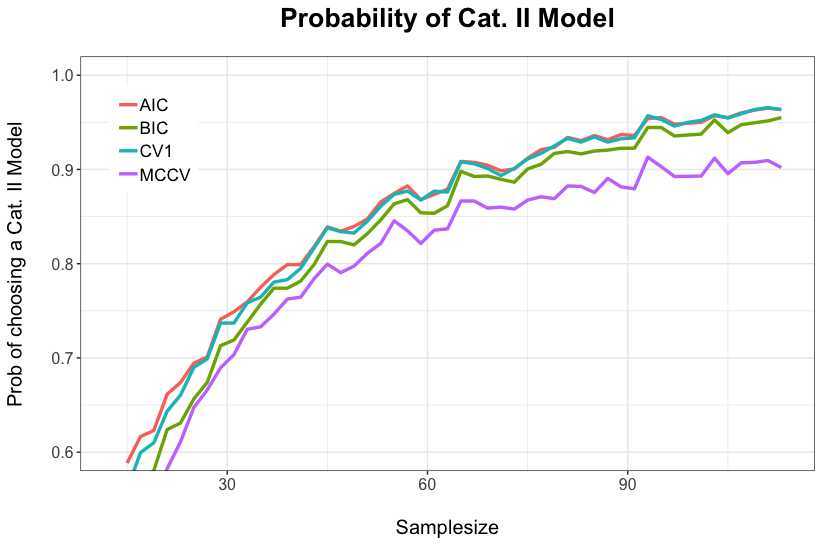
\includegraphics[width=1\textwidth]{Simulation1.png}\\
\caption{Probability of Choosing Cat II Models}
\end{figure}
\subsection{Ability of distinguishing  between Category II Models}
In chapter \ref{Simulation1} we showed that all five methods of model section are quite good in distinguishing between models form Category I and II, hence they all picked Category II models with large probabilities. \\
\\
For the next simulation we only consider models in Category II\footnote{To be more precisely: We only allow Category II models as choice for the model selection problem.}. To rectify this assumption we choose a large sample size of $n=500$, hence we already mentioned that for such large sample size the probability of choosing a Category II model is close to one.\\
\\
Figure \ref{Simulation2} shows the probabilities of choosing models of a certain dimensionality for all five methods\footnote{Therefore we repeated the model selection 2000 times for different samples and counted how often models with certain dimensionality were chosen.}. Since we only look at models from Category II we know that the model with the smallest dimensionality has to be  the true model $M_\ast$. In this sense we denote a model with a dimensionality higher by one then the true models dimensionality with $M_\ast+1$.\\
As we can see, both AIC and CV(1) perform almost equivalent\footnote{These similar performance is not unexpected since \cite{stone1977asymptotic} showed that AIC and CV(1) are asymptotically equivalent} and tend to pick to large models. BIC and MCCV  perform better, both pick the true model with a probability close to one and they choose to large models in only few cases. Within our 2000 simulations there was not a single case where BIC and MCCV chooses models with a dimensionality larger then $M_\ast+1$.
\begin{figure}[!h]
	\label{Simulation2}
	\centering
	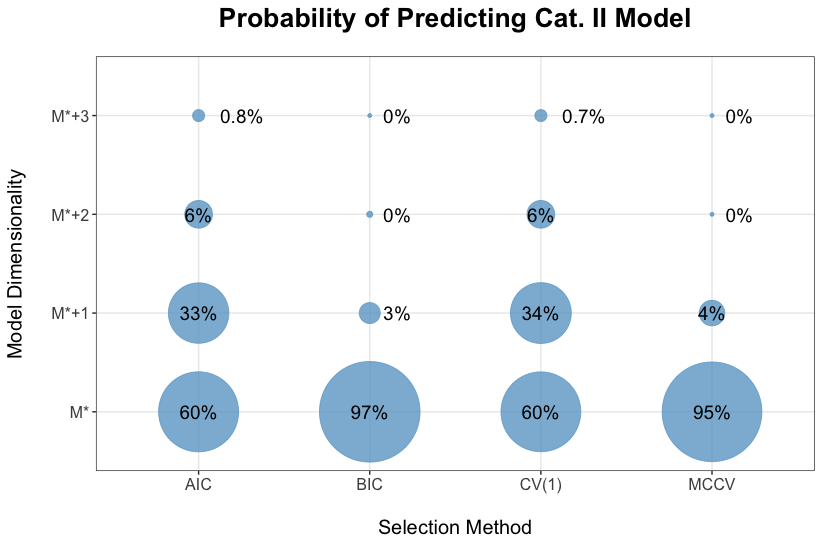
\includegraphics[width=1\textwidth]{Simulation2.png}\\
	\caption{Probability of Choosing diffrent Models form Cat II}
\end{figure}
\subsection{R Code Efficiency}
Beside asymptotic analyses, the performance of the small sample properties is an important aspect of statistical research. An often used approach to analyse such small sample properties are simulation studies, like we did in the previous chapters.\\
\\
Due to inefficiencies of our R code we had to spend weeks of computing time. Therefore one import part of our work was to find ways in order to speed up our R code and reduce it's computational complexity.\\
\\
The most time consuming aspect of our simulations is the process of models selection. As an example consider our CV-algorithm for the case of $n_\nu$=1\footnote{See Rcode in Appendix bla bla bla}: Table \ref{CValt} shows the amount of time used by different R functions within our algorithm.\\
\begin{table}[!h]
	\label{CValt}
	\centering
	\caption{CV Algorithm First Version Profiling }
	\begin{tabular}{lccccc}
		\toprule
		\midrule
		\textbf{\scriptsize }
		&\textbf{\scriptsize self.time}
		&\textbf{\scriptsize self.pct}
		&\textbf{\scriptsize total.time}
		&\textbf{\scriptsize total.pct}
		\\\midrule\midrule
		
		
		\scriptsize as.matrix& \scriptsize 0.44 & \scriptsize 21.15 &\scriptsize 1.28 & \scriptsize 61.54 \\
		\scriptsize CV  &\scriptsize 0.30 & \scriptsize 14.42 &\scriptsize 2.08 & \scriptsize 100 \\
		\scriptsize solved.default & \scriptsize 0.28 & \scriptsize 13.46 &\scriptsize 0.52 & \scriptsize 25 \\
		\scriptsize La.svd  &\scriptsize 0.20 & \scriptsize 9.62 &\scriptsize 0.44 & \scriptsize 21.15 \\
		\scriptsize \%*\% &\scriptsize 0.14 & \scriptsize 6.73 &\scriptsize 0.14& \scriptsize 6.73 \\
		\scriptsize matrix  &\scriptsize 0.12 & \scriptsize 5.77 &\scriptsize 0.18 & \scriptsize 8.65 \\
		\scriptsize t & \scriptsize 0.08 & \scriptsize 3.85 &\scriptsize 0.16 & \scriptsize 7.96 \\
		\scriptsize rownames  &\scriptsize 0.08 & \scriptsize 3.85 &\scriptsize 0.08 & \scriptsize 3.85 \\
		\scriptsize t.default  &\scriptsize 0.08 & \scriptsize 3.85 &\scriptsize 0.08 & \scriptsize 3.85\\
		\scriptsize norm  &\scriptsize 0.06 & \scriptsize 2.88 &\scriptsize 1.78 & \scriptsize  85.58\\
		\scriptsize solve  &\scriptsize  0.06 & \scriptsize 2.88 &\scriptsize 0.74  & \scriptsize 35.58 \\
		\scriptsize  is.atomic &\scriptsize  0.06 & \scriptsize 2.88  &\scriptsize 0.06 & \scriptsize 2.88 \\
		\scriptsize svd  &\scriptsize 0.04 & \scriptsize 1.92  &\scriptsize 1.72  & \scriptsize82.62  \\
		\scriptsize  as.matrix.default &\scriptsize 0.04 & \scriptsize 1.92 &\scriptsize 0.04 & \scriptsize 1.92  \\
		\scriptsize  nrow &\scriptsize 0.04 & \scriptsize 1.92 &\scriptsize 0.04 & \scriptsize  1.92\\
		\scriptsize  colnames <- &\scriptsize  0.02 & \scriptsize 0.96 &\scriptsize 0.04 & \scriptsize 1.92 \\
		\scriptsize  diag &\scriptsize 0.02 & \scriptsize 0.96 &\scriptsize 0.04 & \scriptsize  1.92\\
		\scriptsize is.data.frame  &\scriptsize  0.02 & \scriptsize  0.96 &\scriptsize  0.02& \scriptsize 0.96  \\
		\\
		\scriptsize sampling.time : 2.08
	\end{tabular}
\end{table}
The most time consuming aspects are {\itshape solved.default,\%*\%} and {\itshape t} . All these functions are used for the calculation of the OLS estimators of the diffrent Models in $\mathcal{A}$.
\begin{align*}
\hat{\beta_\alpha}=X_\alpha(X^\prime_\alpha X_\alpha)^{-1}X_\alpha^\prime y
\end{align*}
Note, that we repeat all model selections several times for any fixed $n$ in all simulations. Therefore we generate a complete new sample for each iteration in the simulations and calculate the corresponding OLS estimator. To avoid this we treat X to be deterministic s.t we only have to generate one sample of $X$ observations. In order to introduce stochastic we only use the error term $\varepsilon$ in the data generating process (\ref{SimulationModel}). That means we only have to compute an new $y$ for the different iteration s.t we can pull out the calculation of $X_\alpha(X^\prime_\alpha X_\alpha)^{-1}X_\alpha^\prime$ of the Simulation loop. 

This yields an improvement of speed by a factor of 104 for the new CV-algorithm\footnote{See Code Appendix blabka}. Table \ref{CVneu} shows the time profiling of these new algorithm.\\
\\
\begin{table}[!h]
	\caption{CV Algorithm Second Version Profiling }
	\label{CVneu}
	\centering
	\begin{tabular}{lccccc}
		\toprule
		\midrule
		\textbf{\scriptsize }
		&\textbf{\scriptsize self.time}
		&\textbf{\scriptsize self.pct}
		&\textbf{\scriptsize total.time}
		&\textbf{\scriptsize total.pct}
		\\\midrule\midrule
		\scriptsize tryCatchOne & \scriptsize 0.02 & \scriptsize 100 &\scriptsize 0.02 & \scriptsize 100 \\
		\\
		\scriptsize sampling.time : 0.02
	\end{tabular}
\end{table}
The second approach, to speed R up,  was to look at the basic commands we used and to make them less flexible. To do so we used the command {\itshape package :: function}. This command shows the code behind predefined R commands, for example the {\itshape sample()} command \footnote{{\itshape sample(x,size)} draws randomly {\itshape size} elements from the set {\itshape x} }, see table \ref{sample}.
\begin{table}[h]
	\label{sample}
	\caption{Source Code {\itshape sample()}}
	\begin{lstlisting}
	> base::sample
	function (x, size, replace = FALSE, prob = NULL) 
	{
	if (length(x) == 1L && is.numeric(x) && is.finite(x) && x >= 
	1) {
	if (missing(size)) 
	size <- x
	sample.int(x, size, replace, prob)
	}
	else {
	if (missing(size)) 
	size <- length(x)
	x[sample.int(length(x), size, replace, prob)]	
	}
	}
	\end{lstlisting}
\end{table}
We see that {\itshape sample} checks additional conditions beside it's main purpose, since we do not need this, we can simplify it by using {\itshape x[sample.int(length(x), size)}.\\
\\
One further example is the matrix vector multiplication. R for example would compute $P=X(X^\prime X)^{-1}X^\prime y$ by first solving $X(X^\prime X)^{-1}$, then multiplying the outcome with $X^\prime$ and finally multiplying with $y$. This is inefficient due to the dimensionality of the out coming intermediate results, a more efficient way of computing is $P=X[ (X^\prime X)^{-1}(X^\prime y)]$.
\end{document}